\documentclass{article}
\usepackage{pgfplots}
\pgfplotsset{compat=1.18}
\usepgfplotslibrary{colormaps}

\begin{document}

\begin{figure}[htbp]
  \centering
  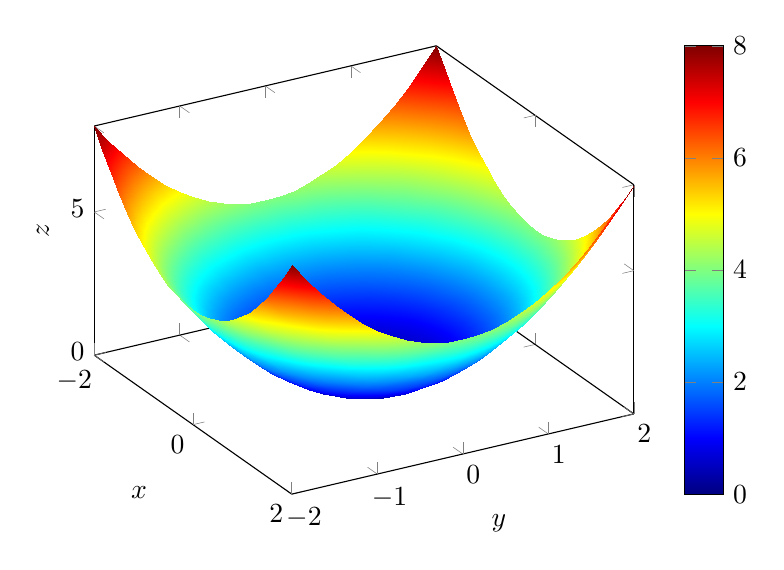
\begin{tikzpicture}
    \begin{axis}[
      xlabel={$x$},
      ylabel={$y$},
      zlabel={$z$},
      colorbar,
      colormap/jet,
      view={60}{35},
      zmin=0, zmax=8,
    ]
      \addplot3[surf, shader=interp, domain=-2:2, y domain=-2:2, samples=25]
        {x^2 + y^2};
    \end{axis}
  \end{tikzpicture}
  \caption{The paraboloid $z = x^2 + y^2$ with a colour bar.}
\end{figure}

\end{document}
